\documentclass[11pt,a4paper]{article}
%\documentclass[11pt,a4paper,twoside]{article}
\usepackage[utf8]{inputenc}
\usepackage[french]{babel}
\usepackage[T1]{fontenc}

\usepackage{amsmath}
\usepackage{amsfonts}
\usepackage{amssymb}

\newcommand{\TitreMatiere}{Architecture des Ordinateurs}
\newcommand{\TitreSeance}{Conversions des Entiers}
\newcommand{\NumeroTD}{non-signés \& signés}
\newcommand{\DateCours}{Novembre 2022}
\newcommand{\AnneeScolaire}{2022-2023}
\newcommand{\Organisation}{EPITA}
\newcommand{\NomAuteurA}{Fabrice BOISSIER}
\newcommand{\MailAuteurA}{fabrice.boissier@epita.fr}
\newcommand{\NomAuteurB}{ }
\newcommand{\MailAuteurB}{ }
\newcommand{\DocKeywords}{Architecture}
\newcommand{\DocLangue}{fr} % "en", "fr", ...

\usepackage{MetalCourseBooklet}

% Babel ne traduit pas toujours bien les tableaux et autres
\renewcommand*\frenchfigurename{%
    {\scshape Figure}%
}
\renewcommand*\frenchtablename{%
    {\scshape Tableau}%
}

% Ne pas afficher le numéro de la légende sur tableaux et figures
\captionsetup{format=sanslabel}


\usepackage{xlop}  % Ajout des jolies divisions posées :   \opdiv{25}{7}  \opidiv{25}{7}
%\usepackage{pstricks}  % style pour xlop

\begin{document}

\EncadreTitre

\bigskip


%\begin{center}
%\begin{tabular}{p{5cm} p{11cm}}
%\textbf{Commandes étudiées :} & \texttt{sh}, \texttt{bash}, \texttt{man}, \texttt{ls}, \texttt{mkdir}, \texttt{touch}, \texttt{chmod}, \texttt{mv}, \texttt{rm}, \texttt{rmdir}, \texttt{cat}, \texttt{file}, \texttt{which}, \texttt{which}\\
%
%\textbf{Builtins étudiées :} & \texttt{pwd}, \texttt{cd}, \texttt{exit}, \texttt{logout}, \texttt{echo}, \texttt{umask}, \texttt{type}, \texttt{>}, \texttt{>{}>}, \texttt{<}, \texttt{<{}<}, \texttt{|}\\
%
%\textbf{Notions étudiées :} & Shell, Manuels, Fichiers, Répertoires, Droits, Redirections\\
%\end{tabular}
%\end{center}

\bigskip


Ce document a pour objectif de vous familiariser avec les conversions entre plusieurs bases dans le cas des entiers non-signés et signés.

\bigskip

La plupart des conversions que nous effectuerons seront entre les bases 2, 8, 10, et 16.

\bigskip

Nous verrons que plusieurs notations existent pour représenter les bases.
Sans symbole particulier, on considère qu'il s'agit de la base 10 usuelle.

\bigskip

%%%%%%%%%%%%%%%%%%%%%%%%%%%%%%%%%%%%%%

\section{Représentation des entiers}

\bigskip

Avant de convertir, particulièrement dans des cas concrets, il est nécessaire de connaître une valeur importante : la \textit{taille des mots} manipulés par le processeur.
En effet, la taille des bus d'adresse et de données sont fondamentales pour savoir quelles valeurs maximum et minimum sont représentables.
Typiquement, un processeur 8 bits ne pourra représenter que 256 valeurs.

Pour comprendre cela, il faut simplement se remémorer les états possibles pour chaque bit, et garder en tête qu'un fil transmet un bit.
Les tableaux suivants vous montre tous les états possibles que peuvent prendre les valeurs sur des bus de 1 bit, 2, bits, 3 bits, et 4 bits.

\begin{table}[h!]
  \centering
  \begin{minipage}{0.45\textwidth}
    \centering

\begin{tabular}{ | m{2cm} | c c c | c | }
\hline
 & \multicolumn{3}{c|}{états} & total\\
\hline
\multirow{2}{*}[0pt]{1 bit} & & & 0 & \multirow{2}{*}[0pt]{2 états} \\
 & & & 1 & \\
\hline
\multirow{4}{*}[0pt]{2 bits} & & 0 & 0 & \multirow{4}{*}[0pt]{4 états} \\
 & & 0 & 1 & \\
 & & 1 & 0 & \\
 & & 1 & 1 & \\
\hline
\multirow{8}{*}[0pt]{3 bits} & 0 & 0 & 0 & \multirow{8}{*}[0pt]{8 états} \\
 & 0 & 0 & 1 & \\
 & 0 & 1 & 0 & \\
 & 0 & 1 & 1 & \\
 & 1 & 0 & 0 & \\
 & 1 & 0 & 1 & \\
 & 1 & 1 & 0 & \\
 & 1 & 1 & 1 & \\
\hline
\end{tabular}

  \end{minipage}
  \hfillx
  \begin{minipage}{0.45\textwidth}
    \centering

\begin{tabular}{ | m{2cm} | c c c c | c | }
\hline
% & \multicolumn{4}{c|}{états} & total\\
%\hline
\multirow{16}{*}[0pt]{4 bits} & 0 & 0 & 0 & 0 & \multirow{16}{*}[0pt]{16 états} \\
 & 0 & 0 & 0 & 1 & \\
 & 0 & 0 & 1 & 0 & \\
 & 0 & 0 & 1 & 1 & \\
 & 0 & 1 & 0 & 0 & \\
 & 0 & 1 & 0 & 1 & \\
 & 0 & 1 & 1 & 0 & \\
 & 0 & 1 & 1 & 1 & \\
 & 1 & 0 & 0 & 0 & \\
 & 1 & 0 & 0 & 1 & \\
 & 1 & 0 & 1 & 0 & \\
 & 1 & 0 & 1 & 1 & \\
 & 1 & 1 & 0 & 0 & \\
 & 1 & 1 & 0 & 1 & \\
 & 1 & 1 & 1 & 0 & \\
 & 1 & 1 & 1 & 1 & \\
\hline
\end{tabular}

  \end{minipage}
%  \caption{Algorithme de la somme des N premiers entiers}
%  \label{somme-n-premiers-entiers}
\end{table}


Vous remarquez intuitivement qu'il s'agit de puissances de $ 2 $ : $ 2^1 = 2 $, $ 2^2 = 4 $, $ 2^3 = 8 $, $ 2^4 = 16 $.
On peut donc déduire le nombre d'états possibles (donc le nombre de valeurs distinctes représentables) avec la formule suivante, où $ N $ représente la taille des mots :

\begin{equation*}
\text{\textit{Nombre d'états possibles}} = 2^{\text{\textit{N}}}
\label{equation:1-Taille-Mots}
\end{equation*}

\bigskip

Une fois la taille des mots fixée, on peut en déduire les valeurs minimales et maximales représentables.
Il existe néanmoins une distinction fondamentale à connaître en architecture : les entiers signés et entiers non-signés.

\begin{itemize}
\item Entiers signés : les entiers sur lesquels le signe est interprété ($ + $ ou $ - $)
\item Entiers non signés : les entiers dont le signe n'est pas utilisé (strictement positifs)
\end{itemize}

On ne fait que manipuler des valeurs où chaque bit sera à $ 0 $ ou $ 1 $, il s'agit donc d'interpréter chacun des états pour qu'il représente une valeur entière.
Chaque \og bit \fg{} (ou fil/pin du processeur) prendra une puissance de $ 2 $, exactement comme pour les dizaines en base 10 :

\medskip

$ 531 =  5 \times 10^2 + 3 \times 10^1 + 1 \times 10^0 $

\smallskip

$ 1010 = 1 \times 2^3 + 0 \times 2^2 + 1 \times 2^1 + 0 \times 2^0 $

\bigskip

Afin de facilement convertir de la base 2 vers la base 10, vous devez connaître par cœur les 10 premières puissances de 10, voire les 13 premières.

\bigskip

\begin{center}
\begin{tabular}{ | c | c c c c c | c c c c c | c c c |}
\hline
$ 2^0 $   &   $ 2^1 $ & $ 2^2 $ & $ 2^3 $ & $ 2^4 $ & $ 2^5 $   &   $ 2^6 $ & $ 2^7 $ & $ 2^8 $ & $ 2^9 $ & $ 2^{10} $   &   $ 2^{11} $ & $ 2^{12} $ & $ 2^{13} $ \\
\hline
$   1 $   &   $   2 $ & $   4 $ & $   8 $ & $  16 $ & $  32 $   &   $  64 $ & $ 128 $ & $ 256 $ & $ 512 $ & $   1024 $   &   $   2048 $ & $   4096 $ & $   8192 $ \\
\hline
\end{tabular}
\end{center}

\bigskip

%%%%%%%%%%%%%%%%%%%%%%%%%%%%%%

\subsection{Entiers non-signés}

\medskip

L'interprétation brut des bits correspond aux entiers non-signés.
Ainsi, sur 8 bits, les entiers non-signés correspondent à :

\bigskip

\begin{center}
\begin{tabular}{ | c | c c c c | c c c c | c |}
\hline
\textit{(base 2)} & $ 2^7 $ & $ 2^6 $ & $ 2^5 $ & $ 2^4 $   &   $ 2^3 $ & $ 2^2 $ & $ 2^1 $ & $ 2^0 $ & \textit{(base 10)} \\
\hline
         & $ 128 $ & $  64 $ & $  32 $ & $  16 $   &   $   8 $ & $   4 $ & $   2 $ & $   1 $ & \\
\hline
0000 0000  &  0 & 0 & 0 & 0  &  0 & 0 & 0 & 0   & 0 \\
0000 0001  &  0 & 0 & 0 & 0  &  0 & 0 & 0 & 1   & 1 \\
0000 0010  &  0 & 0 & 0 & 0  &  0 & 0 & 1 & 0   & 2 \\
0000 0011  &  0 & 0 & 0 & 0  &  0 & 0 & 1 & 1   & 3 \\
0000 0100  &  0 & 0 & 0 & 0  &  0 & 1 & 0 & 0   & 4 \\
0000 0101  &  0 & 0 & 0 & 0  &  0 & 1 & 0 & 1   & 5 \\
0000 0110  &  0 & 0 & 0 & 0  &  0 & 1 & 1 & 0   & 6 \\
0000 0111  &  0 & 0 & 0 & 0  &  0 & 1 & 1 & 1   & 7 \\
0000 1000  &  0 & 0 & 0 & 0  &  1 & 0 & 0 & 0   & 8 \\
... & \multicolumn{4}{|c|}{...} & \multicolumn{4}{c|}{...} & ... \\
0010 0000  &  0 & 0 & 1 & 0  &  0 & 0 & 0 & 0   & 32 \\
0010 0001  &  0 & 0 & 1 & 0  &  0 & 0 & 0 & 1   & 33 \\
... & \multicolumn{4}{|c|}{...} & \multicolumn{4}{c|}{...} & ... \\
0110 0000  &  0 & 1 & 1 & 0  &  0 & 0 & 0 & 0   & 96 \\
0110 0001  &  0 & 1 & 1 & 0  &  0 & 0 & 0 & 1   & 97 \\
0110 0010  &  0 & 1 & 1 & 0  &  0 & 0 & 1 & 0   & 98 \\
0110 0011  &  0 & 1 & 1 & 0  &  0 & 0 & 1 & 1   & 99 \\
0110 0100  &  0 & 1 & 1 & 0  &  0 & 1 & 0 & 0   & 100 \\
... & \multicolumn{4}{|c|}{...} & \multicolumn{4}{c|}{...} & ... \\
1000 0000  &  1 & 0 & 0 & 0  &  0 & 0 & 0 & 0   & 128 \\
... & \multicolumn{4}{|c|}{...} & \multicolumn{4}{c|}{...} & ... \\
1111 1110  &  1 & 1 & 1 & 1  &  1 & 1 & 1 & 0   & 254 \\
1111 1111  &  1 & 1 & 1 & 1  &  1 & 1 & 1 & 1   & 255 \\
\hline
\end{tabular}
\end{center}

\bigskip

Vous vous rendez compte que représenter $ 2^8 $ (256) valeurs  dans le cas non-signé correspond à représenter $ 0 $ et ses 255 suivants.
Ainsi, pour des mots de taille $ N $, les entiers non-signés auront comme borne minimale $ 0 $, et comme borne maximale $ 2^N - 1 $.

\bigskip

%%%%%%%%%%%%%%%%%%%%%%%%%%%%%%

\subsection{Entiers signés}

\medskip

Les entiers signés sont simplement une autre interprétation des données où un bit sert à représenter le signe de l'entier (positif ou négatif).
Une convention est majoritairement utilisée pour représenter les entiers signés : le premier bit sert à coder le signe ($ 0 $ correspond à un nombre positif, et $ 1 $ à un nombre négatif), et on applique le complément à 2 dans le cas négatif.
Ainsi, les entiers signés positifs sont les mêmes que dans le cas des entiers non-signés, mais, il faut d'abord appliquer le complément à 2 à un entier signé négatif pour pouvoir retrouver la valeur absolue binaire.

\bigskip

Appliquer le complément à 2 se résume simplement à appliquer le complément à 1 sur le nombre étudié, puis d'y ajouter $ 1 $.
Le complément à 1 est l'opération visant à intervertir les $ 0 $ par des $ 1 $, et les $ 1 $ par des $ 0 $.

Par exemple, pour appliquer le complément à 2 sur la valeur $ 1001 $ :

\begin{center}
\begin{tabular}{ m{1cm}  c c c c  m{1cm} }
 &  \TTBF{1} & \TTBF{0} & \TTBF{0} & \TTBF{1}  & \\
\end{tabular}

\smallskip

\textit{(complément à 1)}

\smallskip

\begin{tabular}{ m{1cm}  c c c c  m{1cm} }
 &  \TTBF{0} & \TTBF{1} & \TTBF{1} & \TTBF{0}  & \\
\end{tabular}

\smallskip

\textit{(ajout de 1)}

\smallskip

\begin{tabular}{ m{1cm}  c c c c  m{1cm} }
 &  \TTBF{0} & \TTBF{1} & \TTBF{1} & \TTBF{1}  & \\
\end{tabular}
\end{center}

$ 1001 $ correspond donc au négatif de la valeur absolue binaire $ 0111 $ ($ 7 $), c'est-à-dire à $ -7 $.

\bigskip

Ainsi, sur 8 bits, les entiers signés correspondent à :

\bigskip

\begin{center}
\begin{tabular}{ | c | c c c c | c c c c | c | c |}
\hline
\textit{(base 2)} & $ +/- $ & $ 2^6 $ & $ 2^5 $ & $ 2^4 $   &   $ 2^3 $ & $ 2^2 $ & $ 2^1 $ & $ 2^0 $ & \textit{non-signé} & \textit{signé} \\
\hline
         & $ +/- $ & $  64 $ & $  32 $ & $  16 $   &   $   8 $ & $   4 $ & $   2 $ & $   1 $ &       & \\
\hline
1000 0000  &  \textbf{1} & 0 & 0 & 0  &  0 & 0 & 0 & 0   & 128 & -128 \\
1000 0001  &  \textbf{1} & 0 & 0 & 0  &  0 & 0 & 0 & 1   & 129 & -127 \\
1000 0010  &  \textbf{1} & 0 & 0 & 0  &  0 & 0 & 1 & 0   & 130 & -126 \\
1000 0011  &  \textbf{1} & 0 & 0 & 0  &  0 & 0 & 1 & 1   & 131 & -125 \\
... & \multicolumn{4}{c|}{...} & \multicolumn{4}{c|}{...} & ... & ... \\
1001 1001  &  \textbf{1} & 0 & 0 & 1  &  1 & 0 & 0 & 1   & 153 & -103 \\
1001 1010  &  \textbf{1} & 0 & 0 & 1  &  1 & 0 & 1 & 0   & 154 & -102 \\
... & \multicolumn{4}{c|}{...} & \multicolumn{4}{c|}{...} & ... & ... \\
1111 1101  &  \textbf{1} & 1 & 1 & 1  &  1 & 1 & 0 & 1   & 253 & -3 \\
1111 1110  &  \textbf{1} & 1 & 1 & 1  &  1 & 1 & 1 & 0   & 254 & -2 \\
1111 1111  &  \textbf{1} & 1 & 1 & 1  &  1 & 1 & 1 & 1   & 255 & -1 \\
0000 0000  &  \textbf{0} & 0 & 0 & 0  &  0 & 0 & 0 & 0   &   0 & 0 \\
0000 0001  &  \textbf{0} & 0 & 0 & 0  &  0 & 0 & 0 & 1   &   1 & 1 \\
0000 0010  &  \textbf{0} & 0 & 0 & 0  &  0 & 0 & 1 & 0   &   2 & 2 \\
0000 0011  &  \textbf{0} & 0 & 0 & 0  &  0 & 0 & 1 & 1   &   3 & 3 \\
... & \multicolumn{4}{c|}{...} & \multicolumn{4}{c|}{...} & ... & ... \\
0001 1001  &  \textbf{0} & 0 & 0 & 1  &  1 & 0 & 0 & 1   &  25 & 25 \\
0001 1010  &  \textbf{0} & 0 & 0 & 1  &  1 & 0 & 1 & 0   &  26 & 26 \\
... & \multicolumn{4}{c|}{...} & \multicolumn{4}{c|}{...} & ... & ... \\
0111 1100  &  \textbf{0} & 1 & 1 & 1  &  1 & 1 & 0 & 0   & 124 & 124 \\
0111 1101  &  \textbf{0} & 1 & 1 & 1  &  1 & 1 & 0 & 1   & 125 & 125 \\
0111 1110  &  \textbf{0} & 1 & 1 & 1  &  1 & 1 & 1 & 0   & 126 & 126 \\
0111 1111  &  \textbf{0} & 1 & 1 & 1  &  1 & 1 & 1 & 1   & 127 & 127 \\
\hline
\end{tabular}
\end{center}

\bigskip

Vous vous rendez compte que représenter $ 2^8 $ (256) valeurs dans le cas signé correspond à représenter $ 0 $ et ses 127 suivants, ainsi que ses 128 précédents.
Ainsi, pour des mots de taille $ N $, les entiers signés auront comme borne minimale $ - 2^{N-1} $, et comme borne maximale $ 2^{N-1} - 1 $.

Pour conclure, chaque valeur binaire peut être interprétée de différentes manières.

Il est extrêmement important de bien comprendre que \textit{l'interprétation} des valeurs va changer les résultats de certaines opérations !

Comparer sur 8 bits $ 255 $ et $ 0 $ ne donnera pas la même chose si l'on considère les entiers comme signés ou non-signés ($ 0 $ sera le plus petit en mode non-signé, à l'inverse, $ \pm 128 $ sera considéré comme le plus petit en mode signé).

\medskip

%%%%%%%%%%%%%%%%%%%%%%%%%%%%%%

\subsection{Notations des bases}

\medskip

Plusieurs notations pour représenter les bases existent : celles où l'on explicite par un indice en suffixe indiquant dans quelle base celui-ci a été écrit, ou par un caractère en préfixe du nombre.

\begin{itemize}
\item $ 42_{(10)} $ indique l'on écrit le nombre \og $ 42 $ \fg{} en base $ 10 $.
\item $ 0110_{(2)} $ indique que l'on écrit le nombre \og $ 6 $ \fg{} en base $ 2 $, c'est-à-dire $ 0110 $.
\end{itemize}

\medskip

Parmi les caractères servant de préfixe, on retrouvera : $ \%   \; \;  0\text{o}  \; \;  \$  $

\begin{itemize}
\item \og $ \% \, 00101111 $ \fg{} le pourcentage indique que l'on manipule un nombre binaire (ici $ 47 $)
\item \og $ 0\text{o} \, 42 $ \fg{} le zéro suivi d'un O minuscule indiquent que l'on manipule un nombre octal (ici $ 34 $)
\item \og $ \$ \, 15\text{AB} $ \fg{} le dollar indique l'on manipule un nombre hexadécimal (ici $ 5547 $)
\item Un nombre sans préfixe est considéré par défaut comme un nombre décimal.
\end{itemize}

\medskip

%%%%%%%%%%%%%%%%%%%%%%%%%%%%%%%%%%%%%%

\section{Conversions base 2}

\subsection{Base 10 vers 2}

Pour convertir de la base 10 vers la base 2 (également appelée notation binaire), il suffit d'effectuer des divisions successives jusqu'à obtenir $ 1 $.
On reporte ensuite chaque reste, ainsi que le dernier quotient, en bas des divisions successives.
Et enfin, on inverse l'ordre de lecture des chiffres reportés plus bas.

\medskip

%%%%%%%%%%%%%%%%%%%%%%%%%%%%%%%%%%%%%%%%%%%%%%%%%%%%%%%%%%%%%
\begin{center}
\begin{minipage}{6cm}

%% AJOUT POUR FLECHE
\bigskip
\bigskip
\bigskip
\bigskip
\bigskip

%% AJOUT POUR FLECHE
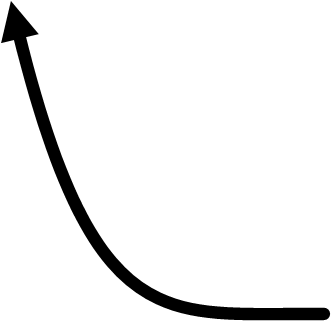
\includegraphics[scale=1]{img/fleche_divisions.png}

%% AJOUT POUR FLECHE
\vspace*{-6cm}

%\opidiv[operandstyle.1=\bfseries,
%        operandstyle.2=\bfseries,
%        remainderstyle.2=\bfseries,
%        remainderstyle.1=\itshape,
%        resultstyle=\bfseries]{42}{2}

\opidiv[remainderstyle.1=\itshape,
        remainderstyle.2=\bfseries]{42}{2}

\leftskip=1cm

\opidiv[remainderstyle.1=\itshape,
        remainderstyle.2=\bfseries]{21}{2}

\leftskip=2cm

\opidiv[remainderstyle.1=\bfseries]{10}{2}

\leftskip=3cm

\opidiv[remainderstyle.1=\bfseries]{5}{2}

\leftskip=3.67cm

\opidiv[remainderstyle.1=\bfseries,
        resultstyle=\bfseries]{2}{2}

\leftskip=0cm

%% AJOUT POUR FLECHE
\vspace{1cm}

\textbf{ \hspace*{0.3cm} 0 \hspace*{0.25cm} 1 \hspace*{0.4cm} 0 \hspace*{0.25cm} 1 \hspace*{0.2cm} 0 | 1}

\end{minipage}
\end{center}
%%%%%%%%%%%%%%%%%%%%%%%%%%%%%%%%%%%%%%%%%%%%%%%%%%%%%%%%%%%%%


Ce qui donne :

\smallskip

{ 0 \hspace*{0.2cm} 1 \hspace*{0.2cm} 0 \hspace*{0.2cm} 1 \hspace*{0.2cm} 0 \hspace*{0.2cm} 1 }

\smallskip

On inverse ensuite l'ordre de lecture en prenant les chiffres depuis la droite (on peut directement lire les résultats des divisions depuis le dernier quotient jusqu'au premier reste en suivant la flèche) :

\smallskip

{ 1 \hspace*{0.2cm} 0 \hspace*{0.2cm} 1 \hspace*{0.2cm} 0 \hspace*{0.2cm} 1 \hspace*{0.2cm} 0 }

\smallskip

Et on obtient ainsi $ 42 $ en binaire, c'est-à-dire : $ \% 101010 $


\bigskip


Pour convertir les nombres négatifs, on applique le même algorithme de conversion vers la base 2, puis on calcule le complément à 2 (c'est-à-dire faire le complément à 1, puis ajouter $ 1 $ au résultat).

\bigskip

Par exemple pour convertir $ -5 $ en base 2 sur 8 bits, on calcule tout d'abord l'équivalent de $ 5 $ en binaire :

\medskip

{ 0 \hspace*{0.2cm} 0 \hspace*{0.2cm} 0 \hspace*{0.2cm} 0 \hspace*{0.2cm} 0 \hspace*{0.2cm} 1 \hspace*{0.2cm} 0 \hspace*{0.2cm} 1 }

\medskip

Puis on calcule son complément à 1 (vous remarquerez que le bit codant le signe passe de $ 0 $ à $ 1 $, indiquant donc maintenant un nombre négatif) :

\medskip

{ 1 \hspace*{0.2cm} 1 \hspace*{0.2cm} 1 \hspace*{0.2cm} 1 \hspace*{0.2cm} 1 \hspace*{0.2cm} 0 \hspace*{0.2cm} 1 \hspace*{0.2cm} 0 }

\medskip

Et enfin on lui ajoute $ 1 $ :

\medskip

{ 1 \hspace*{0.2cm} 1 \hspace*{0.2cm} 1 \hspace*{0.2cm} 1 \hspace*{0.2cm} 1 \hspace*{0.2cm} 0 \hspace*{0.2cm} 1 \hspace*{0.2cm} 1 }

\medskip

Et on obtient ainsi $ -5 $ en binaire sur 8 bits, c'est-à-dire : $ \% \, 1111 \, 1011 $

\bigskip

Pour convertir un nombre négatif en binaire, vous pouvez chercher son ordre de grandeur en base 2 pour déduire combien de chiffres seront nécessaires pour le représenter.
Ensuite, il suffit d'étendre le nombre avec des $ 1 $ devant si la taille des entiers est plus grande (pour les entiers positifs ou non signés, il suffit d'étendre le nombre avec des $ 0 $ devant, comme en base 10).

\bigskip

%%%%%%%%%%%%%%%%%%%%%%%%%%%%%%

\subsection{Base 2 vers 10}

\bigskip

La conversion de la base 2 non-signée vers la base 10 implique simplement d'utiliser la décomposition en puissances de $ 2 $.
On lit chaque chiffre, et on le multiplie par la puissance de $ 2 $ associée.

\bigskip

\begin{tabular}{l c c}
$ \% \, 1010 \; 0110 $  &  $ = $  &  $ 1 \times 2^7 \; + \; 0 \times 2^6 \; + \; 1 \times 2^5 \; + \; 0 \times 2^4  \; \; + \; \; 0 \times 2^3 \; + \; 1 \times 2^2 \; + \; 1 \times 2^1 \; + \; 0 \times 2^0 $ \\
  &  $ = $  &  $ 1 \times 128 \; + \; 0 \times 64 \; + \; 1 \times 32 \; + \; 0 \times 16  \; \; + \; \; 0 \times 8 \; + \; 1 \times 4 \; + \; 1 \times 2 \; + \; 0 \times 1 $ \\
  &  $ = $  &  $ 128 \; + \; 0 \; + \; 32 \; + \; 0 \; \; + \; \; 0 \; + \; 4 \; + \; 2 \; + \; 0 $ \\
%  &  $ = $  &  $ 128 \; + \; 32 \; + \; 4 \; + \; 2 $ \\
  &  $ = $  &  $ 166 $ \\
\end{tabular}

\bigskip

Ainsi, dans le cas d'un entier non-signé, $ \% \, 1010 \; 0110 $ correspond à $ 166 $.

\bigskip

Pour les entiers signés, il suffit de regarder le bit de poids fort (c'est-à-dire le chiffre portant la plus grande valeur, autrement dit, le chiffre le plus à gauche) pour constater qu'il s'agit d'un $ 0 $ (nombre positif) ou d'un $ 1 $ (nombre négatif).
Si le nombre commence par un $ 0 $, et est donc positif, il suffit d'appliquer l'algorithme pour convertir les nombres non-signés.
Si le nombre commence par un $ 1 $, et est donc négatif, il faut donc retirer le bit de poids fort, puis appliquer le complément à 2 avant de convertir avec l'algorithme classique de conversion.

\bigskip

\begin{tabular}{l c c}
$ \% \, \text{\textbf{\underline{1}}}010 \; 0110 $  & & \\
\textit{(nombre négatif)} & & \\
$ \% \, \text{\phantom{1}}010 \; 0110 $  & & \\
\textit{(complément à 1)} & & \\
$ \% \, \text{\phantom{1}}101 \; 1001 $  & & \\
\textit{(ajout de 1)} & & \\
$ \% \, \text{\phantom{1}}101 \; 1010 $  &  $ = $  &  $ 1 \times 2^6 \; + \; 0 \times 2^5 \; + \; 1 \times 2^4  \; \; + \; \; 1 \times 2^3 \; + \; 0 \times 2^2 \; + \; 1 \times 2^1 \; + \; 0 \times 2^0 $ \\
  &  $ = $  &  $ 1 \times 64 \; + \; 0 \times 32 \; + \; 1 \times 16  \; \; + \; \; 1 \times 8 \; + \; 0 \times 4 \; + \; 1 \times 2 \; + \; 0 \times 1 $ \\
  &  $ = $  &  $ 64 \; + \; 0 \; + \; 16 \; \; + \; \; 8 \; + \; 0 \; + \; 2 \; + \; 0 $ \\
%  &  $ = $  &  $ 64 \; + \; 16 \; + \; 8 \; + \; 2 $ \\
  &  $ = $  &  $ 90 $ \\
\textit{(négatif)} & & \\
  &         &  $ - 90 $ \\
\end{tabular}

\bigskip

Ainsi, dans le cas d'un entier signé, $ \% \, 1010 \; 0110 $ correspond à $ -90 $.

\bigskip


%%%%%%%%%%%%%%%%%%%%%%%%%%%%%%%%%%%%%%%%%%%%%%%%%%%

\section{Conversions base 16}

\bigskip

La base 16 (également appelée notation hexadécimale), contrairement à la base 2, étend le nombre de symboles pouvant représenter des données.
Là où la base 2 ne s'appuie que sur deux symboles/deux états possibles, la base 16 s'appuie sur seize symboles/seize états possibles.
Vous devez connaître ces 16 symboles et leurs équivalences en base 10.

\bigskip

\begin{center}
\begin{tabular}{ | c c c c c | c c c c c | c c c c c c | }
\hline
0 & 1 & 2 & 3 & 4  &  5 & 6 & 7 & 8 & 9  &   A &  B &  C &  D &  E &  F \\
\hline
0 & 1 & 2 & 3 & 4  &  5 & 6 & 7 & 8 & 9  &  10 & 11 & 12 & 13 & 14 & 15 \\
\hline
\end{tabular}
\end{center}

\bigskip

%%%%%%%%%%%%%%%%%%%%%%%%%%%%%%

\subsection{Base 10 vers 16}

\bigskip

Pour convertir de la base 10 vers la base 16, il suffit d'effectuer des divisions successives jusqu'à obtenir $ 1 $.
On reporte ensuite chaque reste, ainsi que le dernier quotient, en bas des divisions successives.
Et enfin, on inverse l'ordre de lecture des chiffres reportés plus bas.
La différence avec les divisions par 2 est que lorsque l'on obtient un reste ou un quotient supérieur ou égal à 10, alors on utilise les symboles supplémentaires pour représenter ces valeurs

\bigskip

%%%%%%%%%%%%%%%%%%%%%%%%%%%%%%%%%%%%%%%%%%%%%%%%%%%%%%%%%%%%%
\begin{center}
\begin{minipage}{6cm}

%% AJOUT POUR FLECHE
\bigskip
\bigskip
\bigskip
\bigskip
\bigskip

%% AJOUT POUR FLECHE
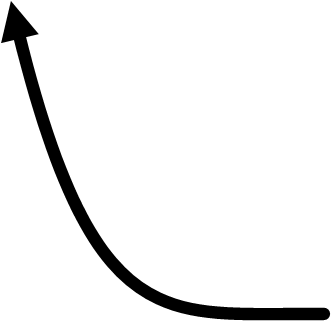
\includegraphics[scale=1]{img/fleche_divisions.png}

%% AJOUT POUR FLECHE
\vspace*{-6cm}

%\opidiv[operandstyle.1=\bfseries,
%        operandstyle.2=\bfseries,
%        remainderstyle.2=\bfseries,
%        remainderstyle.1=\itshape,
%        resultstyle=\bfseries]{42}{2}

\opidiv[remainderstyle.1=\itshape,
        remainderstyle.2=\itshape,
        remainderstyle.3=\itshape,
        remainderstyle.4=\bfseries]{16832}{16}

\leftskip=2cm

\opidiv[remainderstyle.1=\itshape,
        remainderstyle.2=\bfseries]{1052}{16}

\leftskip=3.67cm

\opidiv[remainderstyle.1=\bfseries,
        resultstyle=\bfseries]{65}{16}

\leftskip=3cm

\bigskip

\leftskip=3.67cm

\bigskip

\leftskip=0cm

%% AJOUT POUR FLECHE
\vspace{1cm}

\textbf{ \hspace*{1.15cm} 0 \hspace*{0.75cm} 12 \hspace*{0.6cm} 1 | 4 }

\end{minipage}
\end{center}
%%%%%%%%%%%%%%%%%%%%%%%%%%%%%%%%%%%%%%%%%%%%%%%%%%%%%%%%%%%%%


Ce qui donne :

\medskip

{ 0 \hspace*{0.2cm} 12 \hspace*{0.2cm} 1 \hspace*{0.2cm} 4 }

\medskip

Puis avec la conversion hexadécimale :

\medskip

{ 0 \hspace*{0.2cm} C \hspace*{0.2cm} 1 \hspace*{0.2cm} 4 }

\medskip

On inverse ensuite l'ordre de lecture en prenant les chiffres depuis la droite (on pourrait directement lire les résultats des divisions depuis le dernier quotient jusqu'au premier reste, comme l'indique la flèche) :

\medskip

{ 4 \hspace*{0.2cm} 1 \hspace*{0.2cm} C \hspace*{0.2cm} 0 }

\medskip

Et on obtient ainsi $ 16832 $ en hexadécimal, c'est-à-dire : $ \$ 41\text{C}0 $

\bigskip

Vous constatez que l'algorithme de conversion fonctionne pour plusieurs bases, y compris plus grandes et plus petites que le décimal.
En réalité, cette méthode est l'exacte inverse de la décomposition en puissance de 2 ou 10 (on cherche à obtenir le reste de chaque puissance).

\bigskip

%%%%%%%%%%%%%%%%%%%%%%%%%%%%%%

\subsection{Base 2 vers 16}

\bigskip

Parmi les conversions, vous devez également parfaitement savoir convertir les données binaires en hexadécimal (et inversement).
La méthode de conversion est extrêmement simple, beaucoup plus que les précédentes, car les éléments de la base 16 sont des multiples de la base 2.

\bigskip

Pour convertir des valeurs binaires en valeurs hexadécimales, il suffit simplement de prendre des paquets de 4 bits, et les convertir en un symbole associé.
En effet, sur 4 bits, on peut représenter 16 états, c'est-à-dire que l'on peut utiliser les symboles hexadécimaux pour les écrire.

\bigskip

\begin{tabular}{l c c c c}
$ \% \, 1010 \; 0110 $  &  $ = $  & $ 10 \; \; 6 $ & $ = $ & $ \$ \, \text{A} 6 $ \\
\end{tabular}

\bigskip

On peut directement résumer les valeurs ainsi :

\begin{center}
\begin{tabular}{ | c | c |  m{0.8cm}  | c | c |  m{0.8cm}  | c | c |  m{0.8cm}  | c | c | }
\cline{1-2} \cline{4-5} \cline{7-8} \cline{10-11}
\textit{base 16} & \textit{base 2} & & \textit{base 16} & \textit{base 2} & & \textit{base 16} & \textit{base 2} & & \textit{base 16} & \textit{base 2} \\
\cline{1-2} \cline{4-5} \cline{7-8} \cline{10-11}
0 & 0000 &   & 4 & 0100 &   & 8 & 1000 &   & C & 1100 \\
1 & 0001 &   & 5 & 0101 &   & 9 & 1001 &   & D & 1101 \\
2 & 0010 &   & 6 & 0110 &   & A & 1010 &   & E & 1110 \\
3 & 0011 &   & 7 & 0111 &   & B & 1011 &   & F & 1111 \\
\cline{1-2} \cline{4-5} \cline{7-8} \cline{10-11}
\end{tabular}
\end{center}

\bigskip

Ainsi, que l'entier interprété soit signé ou non-signé, il suffit simplement de transformer les paquets de 4 bits.

%%%%%%%%%%%%%%%%%%%%%%%%%%%%%%

\subsection{Base 16 vers 2}

\bigskip

La conversion dans l'autre sens fonctionne strictement de la même manière : on prend chaque caractère hexadécimal, et on le transforme en son équivalent binaire en conservant l'ordre des chiffres.

\bigskip

\begin{tabular}{l c c c c}
$ \$ \, \text{BA10} $  &  $ = $  & $ 11 \; \; 10 \; \;  1 \; \;  0 $ & $ = $ & $ \% \, 1011 \; 1010 \; 0001 \; 0000 $ \\
$ \$ \, \text{ABCD} $  &  $ = $  & $ 10 \; \; 11 \; \; 12 \; \; 13 $ & $ = $ & $ \% \, 1010 \; 1011 \; 1100 \; 1101 $ \\
$ \$ \, \text{DEAD} $  &  $ = $  & $ 13 \; \; 14 \; \; 10 \; \; 13 $ & $ = $ & $ \% \, 1101 \; 1110 \; 1010 \; 1101 $ \\
$ \$ \, \text{BEEF} $  &  $ = $  & $ 11 \; \; 14 \; \; 14 \; \; 15 $ & $ = $ & $ \% \, 1011 \; 1110 \; 1110 \; 1111 $ \\
\end{tabular}

\bigskip

%%%%%%%%%%%%%%%%%%%%%%%%%%%%%%

\subsection{Base 16 vers 10}

\bigskip

Pour convertir de la base 16 vers la base 10 dans le cas d'un entier non-signé, il suffit de multiplier chaque valeur par la puissance de 16 associée.

\medskip

\begin{tabular}{l c c}
$ \$ \, \text{AD42} $  &  $ = $  &  $ A \times 16^3 \; + \; D \times 16^2 \; + \; 4 \times 16^1 \; + \; 2 \times 16^0 $ \\
  &  $ = $  &  $ 10 \times 4096 \; + \; 14 \times 256 \; + \; 4 \times 16 \; + \; 2 \times 1 $ \\
  &  $ = $  &  $ 40960 \; + \; 3584 \; + \; 64 \; + \; 2 $ \\
  &  $ = $  &  $ 44610 $ \\
\end{tabular}

\medskip

Ainsi, dans le cas d'un entier non-signé, $ \$ \, \text{AD42} $ correspond à $ 44610 $.

\bigskip

Pour convertir un nombre signé, il faut d'abord tester le bit de poids fort pour vérifier s'il est à $ 0 $ ou $ 1 $.
Vous pouvez visuellement savoir cela en regardant la valeur la plus à gauche : si cette valeur est supérieure ou égale à $ 8 $, alors le bit de poids fort sera à $ 1 $, donc le nombre sera négatif.

Dans tous les cas, vous devrez effectuer un complément à 2 sur la valeur binaire.
Pour cette raison, dans le cas des entiers signés dont la valeur la plus à gauche est supérieure ou égale à 8, il vaut mieux convertir le nombre hexadécimal en binaire pour pouvoir faire toutes les opérations suivantes et en déduire le nombre décimal négatif.

\bigskip


%%%%%%%%%%%%%%%%%%%%%%%%%%%%%%%%%%%%%%%%%%%%%%%%%%%

\section{Conversions base 8}

\bigskip

La base 8 (également appelée notation octale) est rarement utilisée, mais il arrive qu'elle le soit.
Vous devez donc savoir convertir la base 8 pour ces quelques situations.
Néanmoins, nous nous contenterons des quelques cas faciles.

\medskip

Comme vous l'avez compris, la base 8 est constituée de chiffres allant de $ 0 $ à $ 7 $.
Ainsi, $ 0\text{o} \, 10 $ correspond à $ 8 $, et $ 0\text{o} \, 21 $ à $ 17 $.

\bigskip

%%%%%%%%%%%%%%%%%%%%%%%%%%%%%%

\subsection{Base 10 vers 8}

\bigskip

Pour convertir de la base 10 vers la base 8, on effectue des divisions successives par $ 8 $ jusqu'à obtenir $ 1 $.

Nous ne montrerons pas d'exemple étant donné que vous maîtrisez maintenant la technique.

\bigskip

%%%%%%%%%%%%%%%%%%%%%%%%%%%%%%

\subsection{Base 8 vers 10}

\bigskip

Pour convertir de la base 8 vers la base 10, il suffit de multiplier par les puissances de 8.

\bigskip

\begin{tabular}{l c c}
$ 0\text{o} \, 4321 $  &  $ = $  &  $ 4 \times 8^3 \; + \; 3 \times 8^2 \; + \; 2 \times 8^1 \; + \; 1 \times 8^0 $ \\
  &  $ = $  &  $ 4 \times 512 \; + \; 3 \times 64 \; + \; 2 \times 16 \; + \; 1 \times 1 $ \\
  &  $ = $  &  $ 2048 \; + \; 192 \; + \; 32 \; + \; 1 $ \\
  &  $ = $  &  $ 2273 $ \\
\end{tabular}

\bigskip

%%%%%%%%%%%%%%%%%%%%%%%%%%%%%%

\subsection{Base 2 vers 8}

\bigskip

Convertir de la base 2 vers de l'octal est extrêmement simple, car la technique est proche de celle de l'hexadécimal.
Au lieu de prendre des paquets de 4 bits (représentants 16 états), il suffit de prendre des paquets de 3 bits (représentants 8 états).

\bigskip

\begin{tabular}{l c c c c c c}
$ \% \, 0111 \; 1010 \; 0110 $  &  $ = $  & $ \% \, 011 \; 110 \; 100 \; 110 $  &  $ = $  & $ 3 \; 6 \; 4 \; 6 $ & $ = $ & $ 0\text{o} \, 3646 $ \\
\end{tabular}

\bigskip

Ainsi, $ \% \, 0111 \; 1010 \; 0110 $ correspond à $ 0\text{o} \, 3646 $, c'est-à-dire $ 1958 $ en décimal.

\bigskip

%%%%%%%%%%%%%%%%%%%%%%%%%%%%%%

\subsection{Base 8 vers 2}

\bigskip

On peut très facilement convertir la base 8 vers la base 2 en exécutant la même démarche précédente inversée : on remplace chaque chiffre par son équivalent binaire.

\bigskip

\begin{tabular}{l c c c c c c}
$ 0\text{o} \, 1337 $  &  $ = $  & $ 1 \; \; 3 \; \;  3 \; \;  7 $ & $ = $ & $ \% \, 001 \; 011 \; 011 \; 111 $ &
                                                                     $ = $ & $ \% \, 0010 \; 1101 \; 1111 $  \\
$ 0\text{o} \, 4321 $  &  $ = $  & $ 4 \; \; 3 \; \;  2 \; \;  1 $ & $ = $ & $ \% \, 100 \; 011 \; 010 \; 001 $ &
                                                                     $ = $ & $ \% \, 1000 \; 1101 \; 0001 $  \\
$ 0\text{o} \, 7065 $  &  $ = $  & $ 7 \; \; 0 \; \;  6 \; \;  5 $ & $ = $ & $ \% \, 111 \; 000 \; 110 \; 101 $ &
                                                                     $ = $ & $ \% \, 1110 \; 0011 \; 0101 $  \\
\end{tabular}

\bigskip



\vfillFirst

\vfillLast

\begin{center}
\textit{Ce document et ses illustrations ont été réalisés par Fabrice BOISSIER en novembre 2022}
\end{center}

\end{document}
